\documentclass{book}
\usepackage[a4paper,top=2.5cm,bottom=2.5cm,left=2.5cm,right=2.5cm]{geometry}
\usepackage{makeidx}
\usepackage{natbib}
\usepackage{graphicx}
\usepackage{multicol}
\usepackage{float}
\usepackage{listings}
\usepackage{color}
\usepackage{ifthen}
\usepackage[table]{xcolor}
\usepackage{textcomp}
\usepackage{alltt}
\usepackage{ifpdf}
\ifpdf
\usepackage[pdftex,
            pagebackref=true,
            colorlinks=true,
            linkcolor=blue,
            unicode
           ]{hyperref}
\else
\usepackage[ps2pdf,
            pagebackref=true,
            colorlinks=true,
            linkcolor=blue,
            unicode
           ]{hyperref}
\usepackage{pspicture}
\fi
\usepackage[utf8]{inputenc}
\usepackage{mathptmx}
\usepackage[scaled=.90]{helvet}
\usepackage{courier}
\usepackage{sectsty}
\usepackage[titles]{tocloft}
\usepackage{doxygen}
\lstset{language=C++,inputencoding=utf8,basicstyle=\footnotesize,breaklines=true,breakatwhitespace=true,tabsize=8,numbers=left }
\makeindex
\setcounter{tocdepth}{3}
\renewcommand{\footrulewidth}{0.4pt}
\renewcommand{\familydefault}{\sfdefault}
\hfuzz=15pt
\setlength{\emergencystretch}{15pt}
\hbadness=750
\tolerance=750
\begin{document}
\hypersetup{pageanchor=false,citecolor=blue}
\begin{titlepage}
\vspace*{7cm}
\begin{center}
{\Large Capstone }\\
\vspace*{1cm}
{\large Generated by Doxygen 1.8.0}\\
\vspace*{0.5cm}
{\small Sun Apr 22 2012 10:38:54}\\
\end{center}
\end{titlepage}
\clearemptydoublepage
\pagenumbering{roman}
\tableofcontents
\clearemptydoublepage
\pagenumbering{arabic}
\hypersetup{pageanchor=true,citecolor=blue}
\chapter{Namespace Index}
\section{Packages}
Here are the packages with brief descriptions (if available)\-:\begin{DoxyCompactList}
\item\contentsline{section}{\hyperlink{namespace_arduino_interface}{Arduino\-Interface} }{\pageref{namespace_arduino_interface}}{}
\item\contentsline{section}{\hyperlink{namespace_database_interface}{Database\-Interface} }{\pageref{namespace_database_interface}}{}
\item\contentsline{section}{\hyperlink{namespace_dump_to_remote}{Dump\-To\-Remote} }{\pageref{namespace_dump_to_remote}}{}
\item\contentsline{section}{\hyperlink{namespace_error}{Error} }{\pageref{namespace_error}}{}
\item\contentsline{section}{\hyperlink{namespace_fill_data}{Fill\-Data} }{\pageref{namespace_fill_data}}{}
\item\contentsline{section}{\hyperlink{namespacegenerator__test_data}{generator\-\_\-test\-Data} }{\pageref{namespacegenerator__test_data}}{}
\item\contentsline{section}{\hyperlink{namespace_gui_interface}{Gui\-Interface} }{\pageref{namespace_gui_interface}}{}
\end{DoxyCompactList}

\chapter{Class Index}
\section{Class Hierarchy}
This inheritance list is sorted roughly, but not completely, alphabetically\-:\begin{DoxyCompactList}
\item \contentsline{section}{Arduino\-Interface.\-Arduino\-Interface}{\pageref{class_arduino_interface_1_1_arduino_interface}}{}
\item \contentsline{section}{Database\-Interface.\-Database\-Interface}{\pageref{class_database_interface_1_1_database_interface}}{}
\begin{DoxyCompactList}
\item \contentsline{section}{Dump\-To\-Remote.\-Dump\-To\-Remote}{\pageref{class_dump_to_remote_1_1_dump_to_remote}}{}
\item \contentsline{section}{Fill\-Data.\-Fill\-Data}{\pageref{class_fill_data_1_1_fill_data}}{}
\end{DoxyCompactList}
\item \contentsline{section}{Error.\-Error}{\pageref{class_error_1_1_error}}{}
\begin{DoxyCompactList}
\item \contentsline{section}{Error.\-arduino\-Error}{\pageref{class_error_1_1arduino_error}}{}
\item \contentsline{section}{Error.\-My\-Error}{\pageref{class_error_1_1_my_error}}{}
\end{DoxyCompactList}
\item \contentsline{section}{Gui\-Interface.\-gui\-Interface}{\pageref{class_gui_interface_1_1gui_interface}}{}
\end{DoxyCompactList}

\chapter{Class Index}
\section{Class List}
Here are the classes, structs, unions and interfaces with brief descriptions\-:\begin{DoxyCompactList}
\item\contentsline{section}{\hyperlink{class_error_1_1arduino_error}{Error.\-arduino\-Error} }{\pageref{class_error_1_1arduino_error}}{}
\item\contentsline{section}{\hyperlink{class_arduino_interface_1_1_arduino_interface}{Arduino\-Interface.\-Arduino\-Interface} }{\pageref{class_arduino_interface_1_1_arduino_interface}}{}
\item\contentsline{section}{\hyperlink{class_database_interface_1_1_database_interface}{Database\-Interface.\-Database\-Interface} }{\pageref{class_database_interface_1_1_database_interface}}{}
\item\contentsline{section}{\hyperlink{class_dump_to_remote_1_1_dump_to_remote}{Dump\-To\-Remote.\-Dump\-To\-Remote} }{\pageref{class_dump_to_remote_1_1_dump_to_remote}}{}
\item\contentsline{section}{\hyperlink{class_error_1_1_error}{Error.\-Error} }{\pageref{class_error_1_1_error}}{}
\item\contentsline{section}{\hyperlink{class_fill_data_1_1_fill_data}{Fill\-Data.\-Fill\-Data} }{\pageref{class_fill_data_1_1_fill_data}}{}
\item\contentsline{section}{\hyperlink{class_gui_interface_1_1gui_interface}{Gui\-Interface.\-gui\-Interface} }{\pageref{class_gui_interface_1_1gui_interface}}{}
\item\contentsline{section}{\hyperlink{class_error_1_1_my_error}{Error.\-My\-Error} }{\pageref{class_error_1_1_my_error}}{}
\end{DoxyCompactList}

\chapter{File Index}
\section{File List}
Here is a list of all files with brief descriptions\-:\begin{DoxyCompactList}
\item\contentsline{section}{A\-:/documents/nathan/\-My Documents/\-Dropbox/\-Workspace/spring2012/\-C\-S495/code/\-Airqual\-Repo/air\-\_\-quality/python\-\_\-src/\hyperlink{_arduino_interface_8py}{Arduino\-Interface.\-py} }{\pageref{_arduino_interface_8py}}{}
\item\contentsline{section}{A\-:/documents/nathan/\-My Documents/\-Dropbox/\-Workspace/spring2012/\-C\-S495/code/\-Airqual\-Repo/air\-\_\-quality/python\-\_\-src/\hyperlink{_database_interface_8py}{Database\-Interface.\-py} }{\pageref{_database_interface_8py}}{}
\item\contentsline{section}{A\-:/documents/nathan/\-My Documents/\-Dropbox/\-Workspace/spring2012/\-C\-S495/code/\-Airqual\-Repo/air\-\_\-quality/python\-\_\-src/\hyperlink{_dump_to_remote_8py}{Dump\-To\-Remote.\-py} }{\pageref{_dump_to_remote_8py}}{}
\item\contentsline{section}{A\-:/documents/nathan/\-My Documents/\-Dropbox/\-Workspace/spring2012/\-C\-S495/code/\-Airqual\-Repo/air\-\_\-quality/python\-\_\-src/\hyperlink{_error_8py}{Error.\-py} }{\pageref{_error_8py}}{}
\item\contentsline{section}{A\-:/documents/nathan/\-My Documents/\-Dropbox/\-Workspace/spring2012/\-C\-S495/code/\-Airqual\-Repo/air\-\_\-quality/python\-\_\-src/\hyperlink{_fill_data_8py}{Fill\-Data.\-py} }{\pageref{_fill_data_8py}}{}
\item\contentsline{section}{A\-:/documents/nathan/\-My Documents/\-Dropbox/\-Workspace/spring2012/\-C\-S495/code/\-Airqual\-Repo/air\-\_\-quality/python\-\_\-src/\hyperlink{generator__test_data_8py}{generator\-\_\-test\-Data.\-py} }{\pageref{generator__test_data_8py}}{}
\item\contentsline{section}{A\-:/documents/nathan/\-My Documents/\-Dropbox/\-Workspace/spring2012/\-C\-S495/code/\-Airqual\-Repo/air\-\_\-quality/python\-\_\-src/\hyperlink{_gui_interface_8py}{Gui\-Interface.\-py} }{\pageref{_gui_interface_8py}}{}
\item\contentsline{section}{A\-:/documents/nathan/\-My Documents/\-Dropbox/\-Workspace/spring2012/\-C\-S495/code/\-Airqual\-Repo/air\-\_\-quality/web\-\_\-src/\hyperlink{_9index_8php}{!index.\-php} }{\pageref{_9index_8php}}{}
\item\contentsline{section}{A\-:/documents/nathan/\-My Documents/\-Dropbox/\-Workspace/spring2012/\-C\-S495/code/\-Airqual\-Repo/air\-\_\-quality/web\-\_\-src/\hyperlink{heatmap_8php}{heatmap.\-php} }{\pageref{heatmap_8php}}{}
\item\contentsline{section}{A\-:/documents/nathan/\-My Documents/\-Dropbox/\-Workspace/spring2012/\-C\-S495/code/\-Airqual\-Repo/air\-\_\-quality/web\-\_\-src/\hyperlink{orig__heatmap_8php}{orig\-\_\-heatmap.\-php} }{\pageref{orig__heatmap_8php}}{}
\item\contentsline{section}{A\-:/documents/nathan/\-My Documents/\-Dropbox/\-Workspace/spring2012/\-C\-S495/code/\-Airqual\-Repo/air\-\_\-quality/web\-\_\-src/\hyperlink{viewdata_8php}{viewdata.\-php} }{\pageref{viewdata_8php}}{}
\item\contentsline{section}{A\-:/documents/nathan/\-My Documents/\-Dropbox/\-Workspace/spring2012/\-C\-S495/code/\-Airqual\-Repo/air\-\_\-quality/web\-\_\-src/phputils/\hyperlink{_9mysqlconnection_8php}{!mysqlconnection.\-php} }{\pageref{_9mysqlconnection_8php}}{}
\item\contentsline{section}{A\-:/documents/nathan/\-My Documents/\-Dropbox/\-Workspace/spring2012/\-C\-S495/code/\-Airqual\-Repo/air\-\_\-quality/web\-\_\-src/phputils/\hyperlink{getdatapoint_8php}{getdatapoint.\-php} }{\pageref{getdatapoint_8php}}{}
\item\contentsline{section}{A\-:/documents/nathan/\-My Documents/\-Dropbox/\-Workspace/spring2012/\-C\-S495/code/\-Airqual\-Repo/air\-\_\-quality/web\-\_\-src/phputils/\hyperlink{mysqlutils_8php}{mysqlutils.\-php} }{\pageref{mysqlutils_8php}}{}
\item\contentsline{section}{A\-:/documents/nathan/\-My Documents/\-Dropbox/\-Workspace/spring2012/\-C\-S495/code/\-Airqual\-Repo/air\-\_\-quality/web\-\_\-src/phputils/\hyperlink{printstaticcontent_8php}{printstaticcontent.\-php} }{\pageref{printstaticcontent_8php}}{}
\end{DoxyCompactList}

\chapter{Namespace Documentation}
\hypertarget{namespace_arduino_interface}{\section{Arduino\-Interface Namespace Reference}
\label{namespace_arduino_interface}\index{Arduino\-Interface@{Arduino\-Interface}}
}
\subsection*{Classes}
\begin{DoxyCompactItemize}
\item 
class \hyperlink{class_arduino_interface_1_1_arduino_interface}{Arduino\-Interface}
\end{DoxyCompactItemize}
\subsection*{Variables}
\begin{DoxyCompactItemize}
\item 
tuple \hyperlink{namespace_arduino_interface_acabd8a3b260b261f4316302aedc34679}{db\-Int} = \hyperlink{class_database_interface_1_1_database_interface}{Database\-Interface.\-Database\-Interface}()
\item 
tuple \hyperlink{namespace_arduino_interface_a755427af9eca690b97c53bf47381365a}{test\-Interface} = \hyperlink{class_arduino_interface_1_1_arduino_interface}{Arduino\-Interface}()
\end{DoxyCompactItemize}


\subsection{Variable Documentation}
\hypertarget{namespace_arduino_interface_acabd8a3b260b261f4316302aedc34679}{\index{Arduino\-Interface@{Arduino\-Interface}!db\-Int@{db\-Int}}
\index{db\-Int@{db\-Int}!ArduinoInterface@{Arduino\-Interface}}
\subsubsection[{db\-Int}]{\setlength{\rightskip}{0pt plus 5cm}tuple {\bf Arduino\-Interface.\-db\-Int} = {\bf Database\-Interface.\-Database\-Interface}()}}\label{namespace_arduino_interface_acabd8a3b260b261f4316302aedc34679}
\hypertarget{namespace_arduino_interface_a755427af9eca690b97c53bf47381365a}{\index{Arduino\-Interface@{Arduino\-Interface}!test\-Interface@{test\-Interface}}
\index{test\-Interface@{test\-Interface}!ArduinoInterface@{Arduino\-Interface}}
\subsubsection[{test\-Interface}]{\setlength{\rightskip}{0pt plus 5cm}tuple {\bf Arduino\-Interface.\-test\-Interface} = {\bf Arduino\-Interface}()}}\label{namespace_arduino_interface_a755427af9eca690b97c53bf47381365a}

\hypertarget{namespace_database_interface}{\section{Database\-Interface Namespace Reference}
\label{namespace_database_interface}\index{Database\-Interface@{Database\-Interface}}
}
\subsection*{Classes}
\begin{DoxyCompactItemize}
\item 
class \hyperlink{class_database_interface_1_1_database_interface}{Database\-Interface}
\end{DoxyCompactItemize}
\subsection*{Variables}
\begin{DoxyCompactItemize}
\item 
tuple \hyperlink{namespace_database_interface_aa4d1de1291859c0a652dc7dc753bcd6f}{test\-Class} = \hyperlink{class_database_interface_1_1_database_interface}{Database\-Interface}()
\end{DoxyCompactItemize}


\subsection{Variable Documentation}
\hypertarget{namespace_database_interface_aa4d1de1291859c0a652dc7dc753bcd6f}{\index{Database\-Interface@{Database\-Interface}!test\-Class@{test\-Class}}
\index{test\-Class@{test\-Class}!DatabaseInterface@{Database\-Interface}}
\subsubsection[{test\-Class}]{\setlength{\rightskip}{0pt plus 5cm}tuple {\bf Database\-Interface.\-test\-Class} = {\bf Database\-Interface}()}}\label{namespace_database_interface_aa4d1de1291859c0a652dc7dc753bcd6f}

\hypertarget{namespace_dump_to_remote}{\section{Dump\-To\-Remote Namespace Reference}
\label{namespace_dump_to_remote}\index{Dump\-To\-Remote@{Dump\-To\-Remote}}
}
\subsection*{Classes}
\begin{DoxyCompactItemize}
\item 
class \hyperlink{class_dump_to_remote_1_1_dump_to_remote}{Dump\-To\-Remote}
\end{DoxyCompactItemize}
\subsection*{Variables}
\begin{DoxyCompactItemize}
\item 
tuple \hyperlink{namespace_dump_to_remote_acf0b6919aa67c6d95dbf0c665a6651c4}{test\-Class} = \hyperlink{class_dump_to_remote_1_1_dump_to_remote}{Dump\-To\-Remote}()
\end{DoxyCompactItemize}


\subsection{Variable Documentation}
\hypertarget{namespace_dump_to_remote_acf0b6919aa67c6d95dbf0c665a6651c4}{\index{Dump\-To\-Remote@{Dump\-To\-Remote}!test\-Class@{test\-Class}}
\index{test\-Class@{test\-Class}!DumpToRemote@{Dump\-To\-Remote}}
\subsubsection[{test\-Class}]{\setlength{\rightskip}{0pt plus 5cm}tuple {\bf Dump\-To\-Remote.\-test\-Class} = {\bf Dump\-To\-Remote}()}}\label{namespace_dump_to_remote_acf0b6919aa67c6d95dbf0c665a6651c4}

\hypertarget{namespace_error}{\section{Error Namespace Reference}
\label{namespace_error}\index{Error@{Error}}
}
\subsection*{Classes}
\begin{DoxyCompactItemize}
\item 
class \hyperlink{class_error_1_1_error}{Error}
\item 
class \hyperlink{class_error_1_1_my_error}{My\-Error}
\item 
class \hyperlink{class_error_1_1arduino_error}{arduino\-Error}
\end{DoxyCompactItemize}

\hypertarget{namespace_fill_data}{\section{Fill\-Data Namespace Reference}
\label{namespace_fill_data}\index{Fill\-Data@{Fill\-Data}}
}
\subsection*{Classes}
\begin{DoxyCompactItemize}
\item 
class \hyperlink{class_fill_data_1_1_fill_data}{Fill\-Data}
\end{DoxyCompactItemize}
\subsection*{Variables}
\begin{DoxyCompactItemize}
\item 
tuple \hyperlink{namespace_fill_data_ab69e8f6937689a4281630e00dceb3bbd}{test\-Class} = \hyperlink{class_fill_data_1_1_fill_data}{Fill\-Data}()
\end{DoxyCompactItemize}


\subsection{Variable Documentation}
\hypertarget{namespace_fill_data_ab69e8f6937689a4281630e00dceb3bbd}{\index{Fill\-Data@{Fill\-Data}!test\-Class@{test\-Class}}
\index{test\-Class@{test\-Class}!FillData@{Fill\-Data}}
\subsubsection[{test\-Class}]{\setlength{\rightskip}{0pt plus 5cm}tuple {\bf Fill\-Data.\-test\-Class} = {\bf Fill\-Data}()}}\label{namespace_fill_data_ab69e8f6937689a4281630e00dceb3bbd}

\hypertarget{namespacegenerator__test_data}{\section{generator\-\_\-test\-Data Namespace Reference}
\label{namespacegenerator__test_data}\index{generator\-\_\-test\-Data@{generator\-\_\-test\-Data}}
}
\subsection*{Functions}
\begin{DoxyCompactItemize}
\item 
def \hyperlink{namespacegenerator__test_data_a4a9465abced90927739acf7a0a515572}{get\-Cursor}
\item 
def \hyperlink{namespacegenerator__test_data_a0e10de95346f6c60ddb26311612e99b4}{create\-Table}
\item 
def \hyperlink{namespacegenerator__test_data_a8aec4184ab35d2a87a24cd5a1f4cdada}{insert\-Data\-Point}
\item 
def \hyperlink{namespacegenerator__test_data_a88f013c3350d785539692899103fa36e}{insert\-Row}
\item 
def \hyperlink{namespacegenerator__test_data_aaa78cde1f9b6b002914b126c91cb1140}{table\-Exists}
\item 
def \hyperlink{namespacegenerator__test_data_a17dd630f225728e09418d808305e93ec}{main}
\end{DoxyCompactItemize}


\subsection{Function Documentation}
\hypertarget{namespacegenerator__test_data_a0e10de95346f6c60ddb26311612e99b4}{\index{generator\-\_\-test\-Data@{generator\-\_\-test\-Data}!create\-Table@{create\-Table}}
\index{create\-Table@{create\-Table}!generator_testData@{generator\-\_\-test\-Data}}
\subsubsection[{create\-Table}]{\setlength{\rightskip}{0pt plus 5cm}def {\bf generator\-\_\-test\-Data.\-create\-Table} (
\begin{DoxyParamCaption}
\item[{}]{data\-Base\-Name, }
\item[{}]{table\-Name}
\end{DoxyParamCaption}
)}}\label{namespacegenerator__test_data_a0e10de95346f6c60ddb26311612e99b4}
\hypertarget{namespacegenerator__test_data_a4a9465abced90927739acf7a0a515572}{\index{generator\-\_\-test\-Data@{generator\-\_\-test\-Data}!get\-Cursor@{get\-Cursor}}
\index{get\-Cursor@{get\-Cursor}!generator_testData@{generator\-\_\-test\-Data}}
\subsubsection[{get\-Cursor}]{\setlength{\rightskip}{0pt plus 5cm}def {\bf generator\-\_\-test\-Data.\-get\-Cursor} (
\begin{DoxyParamCaption}
\item[{}]{data\-Base}
\end{DoxyParamCaption}
)}}\label{namespacegenerator__test_data_a4a9465abced90927739acf7a0a515572}
\hypertarget{namespacegenerator__test_data_a8aec4184ab35d2a87a24cd5a1f4cdada}{\index{generator\-\_\-test\-Data@{generator\-\_\-test\-Data}!insert\-Data\-Point@{insert\-Data\-Point}}
\index{insert\-Data\-Point@{insert\-Data\-Point}!generator_testData@{generator\-\_\-test\-Data}}
\subsubsection[{insert\-Data\-Point}]{\setlength{\rightskip}{0pt plus 5cm}def {\bf generator\-\_\-test\-Data.\-insert\-Data\-Point} (
\begin{DoxyParamCaption}
\item[{}]{gps\-\_\-time, }
\item[{}]{latitude, }
\item[{}]{longitude, }
\item[{}]{co\-\_\-ppm}
\end{DoxyParamCaption}
)}}\label{namespacegenerator__test_data_a8aec4184ab35d2a87a24cd5a1f4cdada}
\hypertarget{namespacegenerator__test_data_a88f013c3350d785539692899103fa36e}{\index{generator\-\_\-test\-Data@{generator\-\_\-test\-Data}!insert\-Row@{insert\-Row}}
\index{insert\-Row@{insert\-Row}!generator_testData@{generator\-\_\-test\-Data}}
\subsubsection[{insert\-Row}]{\setlength{\rightskip}{0pt plus 5cm}def {\bf generator\-\_\-test\-Data.\-insert\-Row} (
\begin{DoxyParamCaption}
\item[{}]{table\-Name, }
\item[{}]{var\-Name, }
\item[{}]{input\-String}
\end{DoxyParamCaption}
)}}\label{namespacegenerator__test_data_a88f013c3350d785539692899103fa36e}
\hypertarget{namespacegenerator__test_data_a17dd630f225728e09418d808305e93ec}{\index{generator\-\_\-test\-Data@{generator\-\_\-test\-Data}!main@{main}}
\index{main@{main}!generator_testData@{generator\-\_\-test\-Data}}
\subsubsection[{main}]{\setlength{\rightskip}{0pt plus 5cm}def {\bf generator\-\_\-test\-Data.\-main} (
\begin{DoxyParamCaption}
{}
\end{DoxyParamCaption}
)}}\label{namespacegenerator__test_data_a17dd630f225728e09418d808305e93ec}
\hypertarget{namespacegenerator__test_data_aaa78cde1f9b6b002914b126c91cb1140}{\index{generator\-\_\-test\-Data@{generator\-\_\-test\-Data}!table\-Exists@{table\-Exists}}
\index{table\-Exists@{table\-Exists}!generator_testData@{generator\-\_\-test\-Data}}
\subsubsection[{table\-Exists}]{\setlength{\rightskip}{0pt plus 5cm}def {\bf generator\-\_\-test\-Data.\-table\-Exists} (
\begin{DoxyParamCaption}
\item[{}]{data\-Base\-Name, }
\item[{}]{table\-Name}
\end{DoxyParamCaption}
)}}\label{namespacegenerator__test_data_aaa78cde1f9b6b002914b126c91cb1140}

\hypertarget{namespace_gui_interface}{\section{Gui\-Interface Namespace Reference}
\label{namespace_gui_interface}\index{Gui\-Interface@{Gui\-Interface}}
}
\subsection*{Classes}
\begin{DoxyCompactItemize}
\item 
class \hyperlink{class_gui_interface_1_1gui_interface}{gui\-Interface}
\end{DoxyCompactItemize}
\subsection*{Variables}
\begin{DoxyCompactItemize}
\item 
tuple \hyperlink{namespace_gui_interface_aad54ad254e54f02b48ef15be00d873db}{test\-Class} = \hyperlink{class_gui_interface_1_1gui_interface}{gui\-Interface}()
\end{DoxyCompactItemize}


\subsection{Variable Documentation}
\hypertarget{namespace_gui_interface_aad54ad254e54f02b48ef15be00d873db}{\index{Gui\-Interface@{Gui\-Interface}!test\-Class@{test\-Class}}
\index{test\-Class@{test\-Class}!GuiInterface@{Gui\-Interface}}
\subsubsection[{test\-Class}]{\setlength{\rightskip}{0pt plus 5cm}tuple {\bf Gui\-Interface.\-test\-Class} = {\bf gui\-Interface}()}}\label{namespace_gui_interface_aad54ad254e54f02b48ef15be00d873db}

\chapter{Class Documentation}
\hypertarget{class_error_1_1arduino_error}{\section{Error.\-arduino\-Error Class Reference}
\label{class_error_1_1arduino_error}\index{Error.\-arduino\-Error@{Error.\-arduino\-Error}}
}
Inheritance diagram for Error.\-arduino\-Error\-:\begin{figure}[H]
\begin{center}
\leavevmode
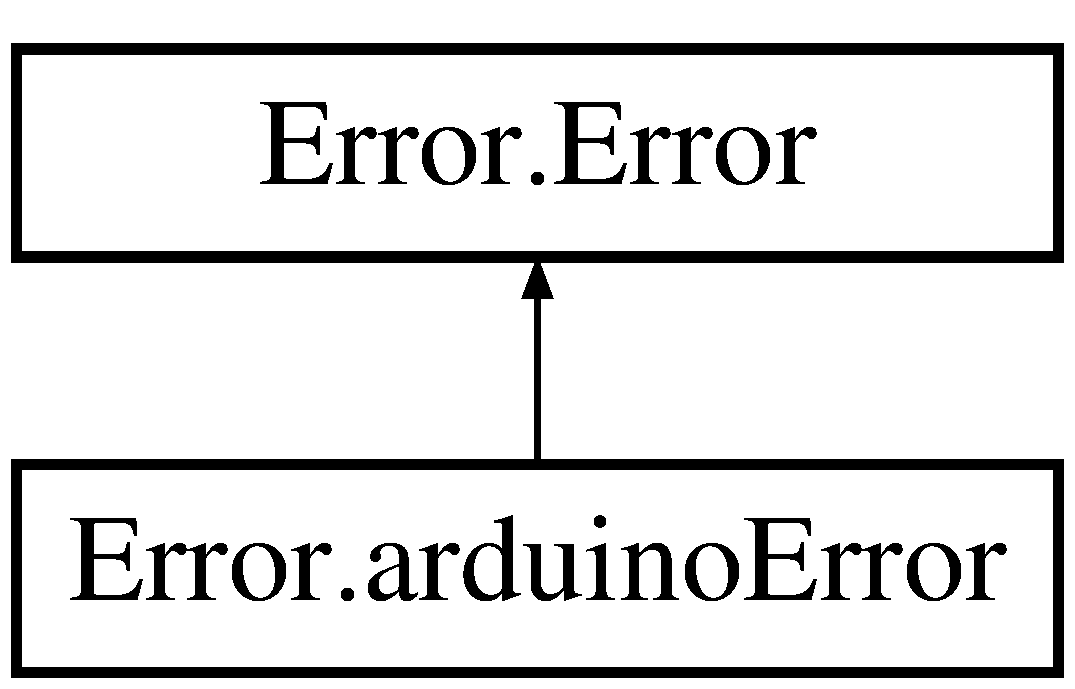
\includegraphics[height=2.000000cm]{class_error_1_1arduino_error}
\end{center}
\end{figure}
\subsection*{Public Member Functions}
\begin{DoxyCompactItemize}
\item 
def \hyperlink{class_error_1_1arduino_error_af4c491b29579c8b181813815e7e8914b}{\-\_\-\-\_\-init\-\_\-\-\_\-}
\end{DoxyCompactItemize}
\subsection*{Public Attributes}
\begin{DoxyCompactItemize}
\item 
\hyperlink{class_error_1_1arduino_error_abd38cfdb82bda4f911c41d018130a3d0}{expr}
\item 
\hyperlink{class_error_1_1arduino_error_aa963133e309f1c2240e98e81d9c092e0}{msg}
\end{DoxyCompactItemize}


\subsection{Constructor \& Destructor Documentation}
\hypertarget{class_error_1_1arduino_error_af4c491b29579c8b181813815e7e8914b}{\index{Error\-::arduino\-Error@{Error\-::arduino\-Error}!\-\_\-\-\_\-init\-\_\-\-\_\-@{\-\_\-\-\_\-init\-\_\-\-\_\-}}
\index{\-\_\-\-\_\-init\-\_\-\-\_\-@{\-\_\-\-\_\-init\-\_\-\-\_\-}!Error::arduinoError@{Error\-::arduino\-Error}}
\subsubsection[{\-\_\-\-\_\-init\-\_\-\-\_\-}]{\setlength{\rightskip}{0pt plus 5cm}def {\bf Error.\-arduino\-Error.\-\_\-\-\_\-init\-\_\-\-\_\-} (
\begin{DoxyParamCaption}
\item[{}]{self, }
\item[{}]{expr, }
\item[{}]{msg}
\end{DoxyParamCaption}
)}}\label{class_error_1_1arduino_error_af4c491b29579c8b181813815e7e8914b}


\subsection{Member Data Documentation}
\hypertarget{class_error_1_1arduino_error_abd38cfdb82bda4f911c41d018130a3d0}{\index{Error\-::arduino\-Error@{Error\-::arduino\-Error}!expr@{expr}}
\index{expr@{expr}!Error::arduinoError@{Error\-::arduino\-Error}}
\subsubsection[{expr}]{\setlength{\rightskip}{0pt plus 5cm}{\bf Error.\-arduino\-Error.\-expr}}}\label{class_error_1_1arduino_error_abd38cfdb82bda4f911c41d018130a3d0}
\hypertarget{class_error_1_1arduino_error_aa963133e309f1c2240e98e81d9c092e0}{\index{Error\-::arduino\-Error@{Error\-::arduino\-Error}!msg@{msg}}
\index{msg@{msg}!Error::arduinoError@{Error\-::arduino\-Error}}
\subsubsection[{msg}]{\setlength{\rightskip}{0pt plus 5cm}{\bf Error.\-arduino\-Error.\-msg}}}\label{class_error_1_1arduino_error_aa963133e309f1c2240e98e81d9c092e0}


The documentation for this class was generated from the following file\-:\begin{DoxyCompactItemize}
\item 
A\-:/documents/nathan/\-My Documents/\-Dropbox/\-Workspace/spring2012/\-C\-S495/code/\-Airqual\-Repo/air\-\_\-quality/python\-\_\-src/\hyperlink{_error_8py}{Error.\-py}\end{DoxyCompactItemize}

\hypertarget{class_arduino_interface_1_1_arduino_interface}{\section{Arduino\-Interface.\-Arduino\-Interface Class Reference}
\label{class_arduino_interface_1_1_arduino_interface}\index{Arduino\-Interface.\-Arduino\-Interface@{Arduino\-Interface.\-Arduino\-Interface}}
}
\subsection*{Public Member Functions}
\begin{DoxyCompactItemize}
\item 
\hypertarget{class_arduino_interface_1_1_arduino_interface_ad0063b90161fa8323cef433a13bb6e8b}{def {\bfseries \-\_\-\-\_\-init\-\_\-\-\_\-}}\label{class_arduino_interface_1_1_arduino_interface_ad0063b90161fa8323cef433a13bb6e8b}

\item 
\hypertarget{class_arduino_interface_1_1_arduino_interface_aa292ce6b4406b3e975e703502cca0e39}{def {\bfseries send\-Data}}\label{class_arduino_interface_1_1_arduino_interface_aa292ce6b4406b3e975e703502cca0e39}

\item 
\hypertarget{class_arduino_interface_1_1_arduino_interface_ae1ac3ad21ffe702a7b97ac3e05a22fc0}{def {\bfseries get\-Data}}\label{class_arduino_interface_1_1_arduino_interface_ae1ac3ad21ffe702a7b97ac3e05a22fc0}

\item 
\hypertarget{class_arduino_interface_1_1_arduino_interface_af07f9f858c6274d9cc1247c7dd14ebf6}{def {\bfseries print\-Serial}}\label{class_arduino_interface_1_1_arduino_interface_af07f9f858c6274d9cc1247c7dd14ebf6}

\item 
\hypertarget{class_arduino_interface_1_1_arduino_interface_a0e311cf3263799415c2ff536c7b42cf8}{def {\bfseries get\-Connection}}\label{class_arduino_interface_1_1_arduino_interface_a0e311cf3263799415c2ff536c7b42cf8}

\item 
\hypertarget{class_arduino_interface_1_1_arduino_interface_ac215fb8000c089a566d70f1b59c272b3}{def {\bfseries main}}\label{class_arduino_interface_1_1_arduino_interface_ac215fb8000c089a566d70f1b59c272b3}

\end{DoxyCompactItemize}


The documentation for this class was generated from the following file\-:\begin{DoxyCompactItemize}
\item 
C\-:/\-Users/nathan.\-boyd/\-Dropbox/\-Workspace/spring2012/\-C\-S495/code/\-Airqual\-Repo/air\-\_\-quality/python\-\_\-src/Arduino\-Interface.\-py\end{DoxyCompactItemize}

\hypertarget{class_database_interface_1_1_database_interface}{\section{Database\-Interface.\-Database\-Interface Class Reference}
\label{class_database_interface_1_1_database_interface}\index{Database\-Interface.\-Database\-Interface@{Database\-Interface.\-Database\-Interface}}
}
Inheritance diagram for Database\-Interface.\-Database\-Interface\-:\begin{figure}[H]
\begin{center}
\leavevmode
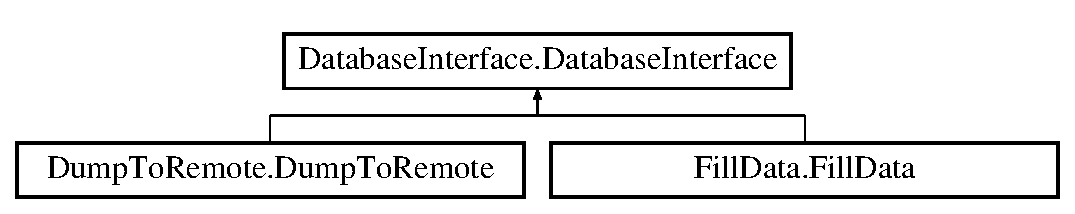
\includegraphics[height=2.000000cm]{class_database_interface_1_1_database_interface}
\end{center}
\end{figure}
\subsection*{Public Member Functions}
\begin{DoxyCompactItemize}
\item 
\hypertarget{class_database_interface_1_1_database_interface_a79b2f185cf35d225238e22921254ba0f}{def {\bfseries \-\_\-\-\_\-init\-\_\-\-\_\-}}\label{class_database_interface_1_1_database_interface_a79b2f185cf35d225238e22921254ba0f}

\item 
\hypertarget{class_database_interface_1_1_database_interface_a9c7a69525645d39f1d2967b2221b0e95}{def {\bfseries get\-Cursor}}\label{class_database_interface_1_1_database_interface_a9c7a69525645d39f1d2967b2221b0e95}

\item 
\hypertarget{class_database_interface_1_1_database_interface_a403157af3a4e682ce0244a59885980e3}{def {\bfseries create\-Table}}\label{class_database_interface_1_1_database_interface_a403157af3a4e682ce0244a59885980e3}

\item 
\hypertarget{class_database_interface_1_1_database_interface_a0cdcada6026e9de3ef363e7ffe43a055}{def {\bfseries table\-Exists}}\label{class_database_interface_1_1_database_interface_a0cdcada6026e9de3ef363e7ffe43a055}

\item 
\hypertarget{class_database_interface_1_1_database_interface_a62f0ccdb9b87ae7fd37f57058177b29b}{def {\bfseries insert\-Data\-Point}}\label{class_database_interface_1_1_database_interface_a62f0ccdb9b87ae7fd37f57058177b29b}

\item 
\hypertarget{class_database_interface_1_1_database_interface_a5ce1c3e2d2da9cfc3e51162f8ce00e63}{def {\bfseries insert\-Row}}\label{class_database_interface_1_1_database_interface_a5ce1c3e2d2da9cfc3e51162f8ce00e63}

\item 
\hypertarget{class_database_interface_1_1_database_interface_a34cd488b227a7742298c622a70511ae1}{def {\bfseries main}}\label{class_database_interface_1_1_database_interface_a34cd488b227a7742298c622a70511ae1}

\end{DoxyCompactItemize}
\subsection*{Static Public Attributes}
\begin{DoxyCompactItemize}
\item 
\hypertarget{class_database_interface_1_1_database_interface_ac0a2837d86558a1bfe62834dcd6274f3}{string {\bfseries W\-O\-R\-K\-I\-N\-G\-\_\-\-D\-B} = 'local'}\label{class_database_interface_1_1_database_interface_ac0a2837d86558a1bfe62834dcd6274f3}

\item 
\hypertarget{class_database_interface_1_1_database_interface_ae92289621f90ec296eb0cd89b9f6fc91}{{\bfseries D\-E\-B\-U\-G} = False}\label{class_database_interface_1_1_database_interface_ae92289621f90ec296eb0cd89b9f6fc91}

\end{DoxyCompactItemize}


The documentation for this class was generated from the following file\-:\begin{DoxyCompactItemize}
\item 
C\-:/\-Users/nathan.\-boyd/\-Dropbox/\-Workspace/spring2012/\-C\-S495/code/\-Airqual\-Repo/air\-\_\-quality/python\-\_\-src/Database\-Interface.\-py\end{DoxyCompactItemize}

\hypertarget{class_dump_to_remote_1_1_dump_to_remote}{\section{Dump\-To\-Remote.\-Dump\-To\-Remote Class Reference}
\label{class_dump_to_remote_1_1_dump_to_remote}\index{Dump\-To\-Remote.\-Dump\-To\-Remote@{Dump\-To\-Remote.\-Dump\-To\-Remote}}
}
Inheritance diagram for Dump\-To\-Remote.\-Dump\-To\-Remote\-:\begin{figure}[H]
\begin{center}
\leavevmode
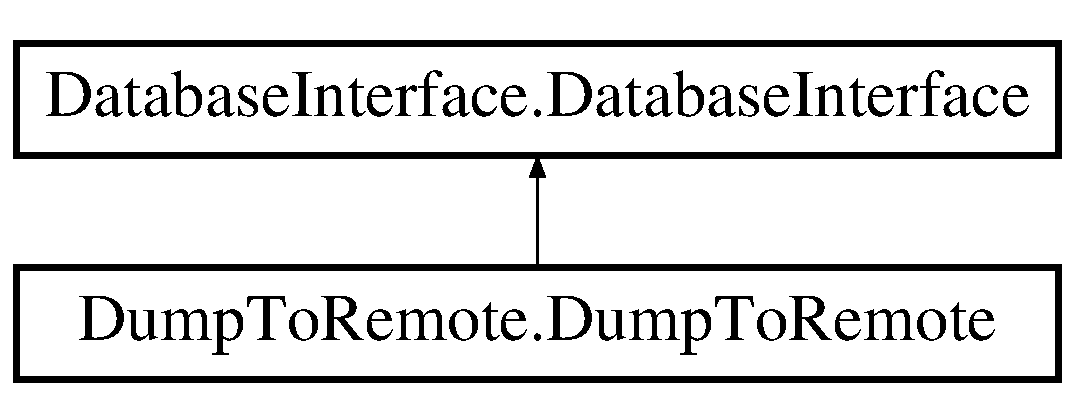
\includegraphics[height=2.000000cm]{class_dump_to_remote_1_1_dump_to_remote}
\end{center}
\end{figure}
\subsection*{Public Member Functions}
\begin{DoxyCompactItemize}
\item 
\hypertarget{class_dump_to_remote_1_1_dump_to_remote_ad564941589b93a68ff46498cc21da2f2}{def {\bfseries \-\_\-\-\_\-init\-\_\-\-\_\-}}\label{class_dump_to_remote_1_1_dump_to_remote_ad564941589b93a68ff46498cc21da2f2}

\item 
\hypertarget{class_dump_to_remote_1_1_dump_to_remote_adb91f51d25a482426704c6a0c0c1377f}{def {\bfseries main}}\label{class_dump_to_remote_1_1_dump_to_remote_adb91f51d25a482426704c6a0c0c1377f}

\end{DoxyCompactItemize}


The documentation for this class was generated from the following file\-:\begin{DoxyCompactItemize}
\item 
C\-:/\-Users/nathan.\-boyd/\-Dropbox/\-Workspace/spring2012/\-C\-S495/code/\-Airqual\-Repo/air\-\_\-quality/python\-\_\-src/Dump\-To\-Remote.\-py\end{DoxyCompactItemize}

\hypertarget{class_error_1_1_error}{\section{Error.\-Error Class Reference}
\label{class_error_1_1_error}\index{Error.\-Error@{Error.\-Error}}
}
Inheritance diagram for Error.\-Error\-:\begin{figure}[H]
\begin{center}
\leavevmode
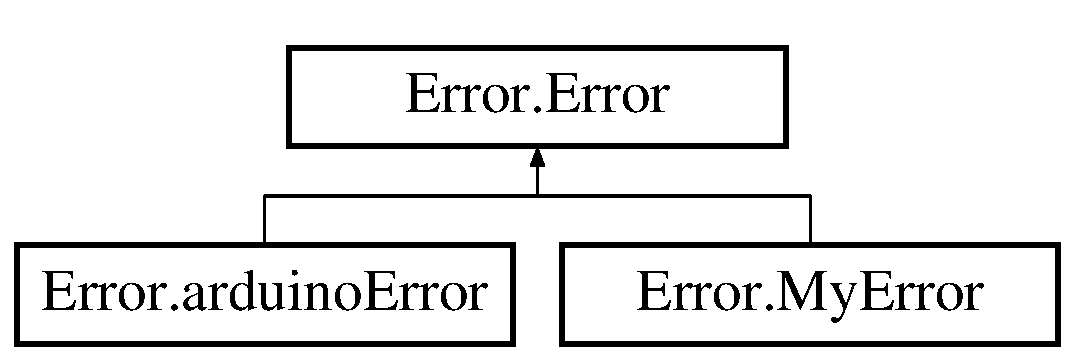
\includegraphics[height=2.000000cm]{class_error_1_1_error}
\end{center}
\end{figure}


\subsection{Detailed Description}
\begin{DoxyVerb}Base class for exceptions in this module.\end{DoxyVerb}
 

The documentation for this class was generated from the following file\-:\begin{DoxyCompactItemize}
\item 
A\-:/documents/nathan/\-My Documents/\-Dropbox/\-Workspace/spring2012/\-C\-S495/code/\-Airqual\-Repo/air\-\_\-quality/python\-\_\-src/\hyperlink{_error_8py}{Error.\-py}\end{DoxyCompactItemize}

\hypertarget{class_fill_data_1_1_fill_data}{\section{Fill\-Data.\-Fill\-Data Class Reference}
\label{class_fill_data_1_1_fill_data}\index{Fill\-Data.\-Fill\-Data@{Fill\-Data.\-Fill\-Data}}
}
Inheritance diagram for Fill\-Data.\-Fill\-Data\-:\begin{figure}[H]
\begin{center}
\leavevmode
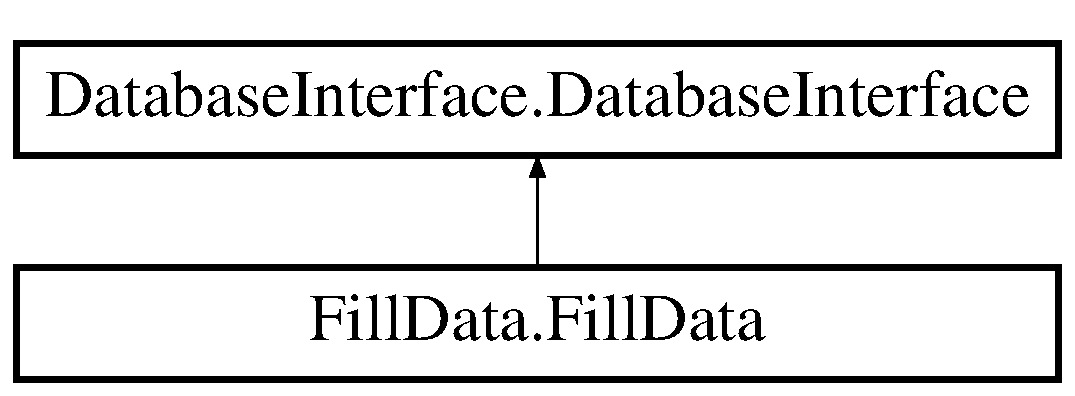
\includegraphics[height=2.000000cm]{class_fill_data_1_1_fill_data}
\end{center}
\end{figure}
\subsection*{Public Member Functions}
\begin{DoxyCompactItemize}
\item 
\hypertarget{class_fill_data_1_1_fill_data_af740b6816f2b16d11688251cbd0eefff}{def {\bfseries \-\_\-\-\_\-init\-\_\-\-\_\-}}\label{class_fill_data_1_1_fill_data_af740b6816f2b16d11688251cbd0eefff}

\item 
\hypertarget{class_fill_data_1_1_fill_data_acce1c8c84567e2e1cf45e0160d80006e}{def {\bfseries check\-Townships}}\label{class_fill_data_1_1_fill_data_acce1c8c84567e2e1cf45e0160d80006e}

\item 
\hypertarget{class_fill_data_1_1_fill_data_af9c92e35e375bed232be9bec5bce5ad0}{def {\bfseries check\-Addresses}}\label{class_fill_data_1_1_fill_data_af9c92e35e375bed232be9bec5bce5ad0}

\item 
\hypertarget{class_fill_data_1_1_fill_data_a8a24290464e37b6f668338c7b75dab69}{def {\bfseries main}}\label{class_fill_data_1_1_fill_data_a8a24290464e37b6f668338c7b75dab69}

\end{DoxyCompactItemize}


The documentation for this class was generated from the following file\-:\begin{DoxyCompactItemize}
\item 
C\-:/\-Users/nathan.\-boyd/\-Dropbox/\-Workspace/spring2012/\-C\-S495/code/\-Airqual\-Repo/air\-\_\-quality/python\-\_\-src/Fill\-Data.\-py\end{DoxyCompactItemize}

\hypertarget{class_gui_interface_1_1gui_interface}{\section{Gui\-Interface.\-gui\-Interface Class Reference}
\label{class_gui_interface_1_1gui_interface}\index{Gui\-Interface.\-gui\-Interface@{Gui\-Interface.\-gui\-Interface}}
}
\subsection*{Public Member Functions}
\begin{DoxyCompactItemize}
\item 
def \hyperlink{class_gui_interface_1_1gui_interface_ac54648b04404d73cdf5cc648cd0df814}{start\-Sensor}
\item 
def \hyperlink{class_gui_interface_1_1gui_interface_a87f803203fddf02263f7edf07e47097a}{fill\-Locality}
\item 
def \hyperlink{class_gui_interface_1_1gui_interface_a64d4c8bc5d86f421303bddf0d12d18f3}{dump\-To\-Remote}
\item 
def \hyperlink{class_gui_interface_1_1gui_interface_a57f43b82011bb65e63628118e023b748}{main}
\end{DoxyCompactItemize}


\subsection{Member Function Documentation}
\hypertarget{class_gui_interface_1_1gui_interface_a64d4c8bc5d86f421303bddf0d12d18f3}{\index{Gui\-Interface\-::gui\-Interface@{Gui\-Interface\-::gui\-Interface}!dump\-To\-Remote@{dump\-To\-Remote}}
\index{dump\-To\-Remote@{dump\-To\-Remote}!GuiInterface::guiInterface@{Gui\-Interface\-::gui\-Interface}}
\subsubsection[{dump\-To\-Remote}]{\setlength{\rightskip}{0pt plus 5cm}def {\bf Gui\-Interface.\-gui\-Interface.\-dump\-To\-Remote} (
\begin{DoxyParamCaption}
\item[{}]{self}
\end{DoxyParamCaption}
)}}\label{class_gui_interface_1_1gui_interface_a64d4c8bc5d86f421303bddf0d12d18f3}
\hypertarget{class_gui_interface_1_1gui_interface_a87f803203fddf02263f7edf07e47097a}{\index{Gui\-Interface\-::gui\-Interface@{Gui\-Interface\-::gui\-Interface}!fill\-Locality@{fill\-Locality}}
\index{fill\-Locality@{fill\-Locality}!GuiInterface::guiInterface@{Gui\-Interface\-::gui\-Interface}}
\subsubsection[{fill\-Locality}]{\setlength{\rightskip}{0pt plus 5cm}def {\bf Gui\-Interface.\-gui\-Interface.\-fill\-Locality} (
\begin{DoxyParamCaption}
\item[{}]{self}
\end{DoxyParamCaption}
)}}\label{class_gui_interface_1_1gui_interface_a87f803203fddf02263f7edf07e47097a}
\hypertarget{class_gui_interface_1_1gui_interface_a57f43b82011bb65e63628118e023b748}{\index{Gui\-Interface\-::gui\-Interface@{Gui\-Interface\-::gui\-Interface}!main@{main}}
\index{main@{main}!GuiInterface::guiInterface@{Gui\-Interface\-::gui\-Interface}}
\subsubsection[{main}]{\setlength{\rightskip}{0pt plus 5cm}def {\bf Gui\-Interface.\-gui\-Interface.\-main} (
\begin{DoxyParamCaption}
\item[{}]{self}
\end{DoxyParamCaption}
)}}\label{class_gui_interface_1_1gui_interface_a57f43b82011bb65e63628118e023b748}
\hypertarget{class_gui_interface_1_1gui_interface_ac54648b04404d73cdf5cc648cd0df814}{\index{Gui\-Interface\-::gui\-Interface@{Gui\-Interface\-::gui\-Interface}!start\-Sensor@{start\-Sensor}}
\index{start\-Sensor@{start\-Sensor}!GuiInterface::guiInterface@{Gui\-Interface\-::gui\-Interface}}
\subsubsection[{start\-Sensor}]{\setlength{\rightskip}{0pt plus 5cm}def {\bf Gui\-Interface.\-gui\-Interface.\-start\-Sensor} (
\begin{DoxyParamCaption}
\item[{}]{self}
\end{DoxyParamCaption}
)}}\label{class_gui_interface_1_1gui_interface_ac54648b04404d73cdf5cc648cd0df814}


The documentation for this class was generated from the following file\-:\begin{DoxyCompactItemize}
\item 
A\-:/documents/nathan/\-My Documents/\-Dropbox/\-Workspace/spring2012/\-C\-S495/code/\-Airqual\-Repo/air\-\_\-quality/python\-\_\-src/\hyperlink{_gui_interface_8py}{Gui\-Interface.\-py}\end{DoxyCompactItemize}

\hypertarget{class_error_1_1_my_error}{\section{Error.\-My\-Error Class Reference}
\label{class_error_1_1_my_error}\index{Error.\-My\-Error@{Error.\-My\-Error}}
}
Inheritance diagram for Error.\-My\-Error\-:\begin{figure}[H]
\begin{center}
\leavevmode
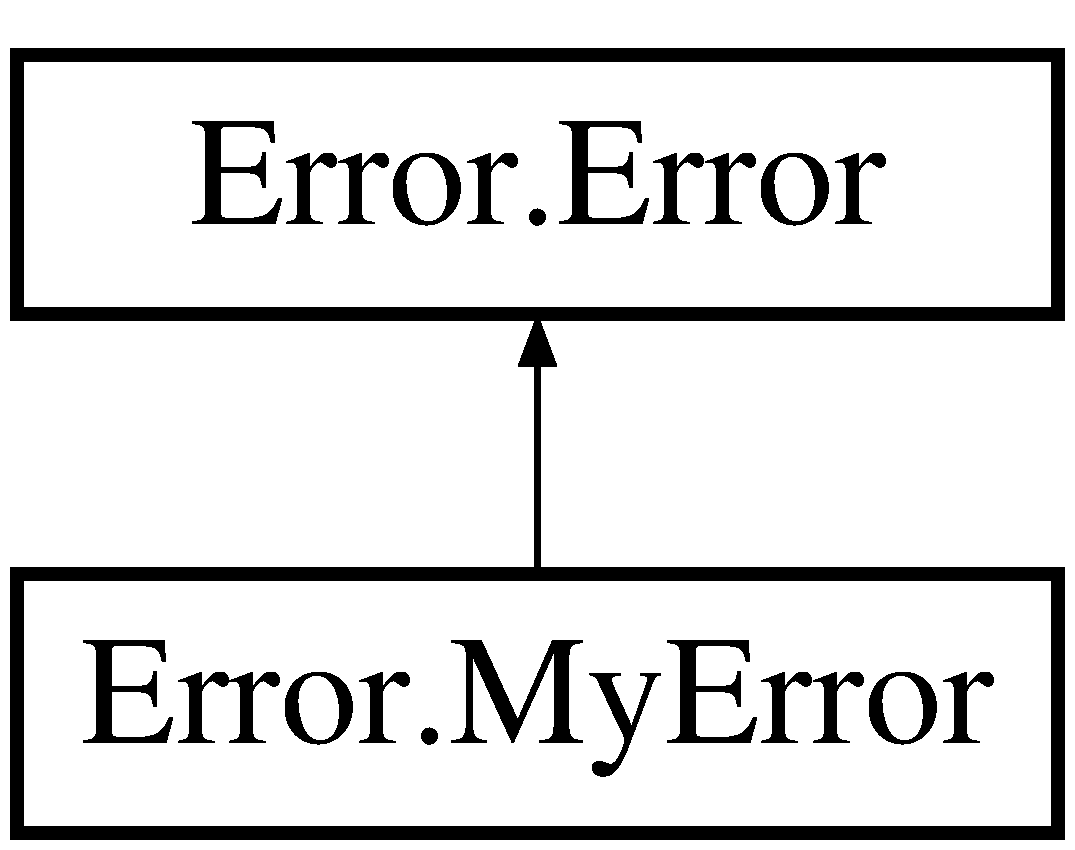
\includegraphics[height=2.000000cm]{class_error_1_1_my_error}
\end{center}
\end{figure}
\subsection*{Public Member Functions}
\begin{DoxyCompactItemize}
\item 
\hypertarget{class_error_1_1_my_error_a7a269ccbf9182b2a818d1a33c0436bce}{def {\bfseries \-\_\-\-\_\-init\-\_\-\-\_\-}}\label{class_error_1_1_my_error_a7a269ccbf9182b2a818d1a33c0436bce}

\item 
\hypertarget{class_error_1_1_my_error_a7ce4fb2ab3d7e6ef6a393c4e09c99618}{def {\bfseries \-\_\-\-\_\-str\-\_\-\-\_\-}}\label{class_error_1_1_my_error_a7ce4fb2ab3d7e6ef6a393c4e09c99618}

\end{DoxyCompactItemize}
\subsection*{Public Attributes}
\begin{DoxyCompactItemize}
\item 
\hypertarget{class_error_1_1_my_error_a768d5e180ecca5aaf742c1389dcfeb00}{{\bfseries value}}\label{class_error_1_1_my_error_a768d5e180ecca5aaf742c1389dcfeb00}

\end{DoxyCompactItemize}


The documentation for this class was generated from the following file\-:\begin{DoxyCompactItemize}
\item 
C\-:/\-Users/nathan.\-boyd/\-Dropbox/\-Workspace/spring2012/\-C\-S495/code/\-Airqual\-Repo/air\-\_\-quality/python\-\_\-src/Error.\-py\end{DoxyCompactItemize}

\chapter{File Documentation}
\hypertarget{_arduino_interface_8py}{\section{A\-:/documents/nathan/\-My Documents/\-Dropbox/\-Workspace/spring2012/\-C\-S495/code/\-Airqual\-Repo/air\-\_\-quality/python\-\_\-src/\-Arduino\-Interface.py File Reference}
\label{_arduino_interface_8py}\index{A\-:/documents/nathan/\-My Documents/\-Dropbox/\-Workspace/spring2012/\-C\-S495/code/\-Airqual\-Repo/air\-\_\-quality/python\-\_\-src/\-Arduino\-Interface.\-py@{A\-:/documents/nathan/\-My Documents/\-Dropbox/\-Workspace/spring2012/\-C\-S495/code/\-Airqual\-Repo/air\-\_\-quality/python\-\_\-src/\-Arduino\-Interface.\-py}}
}
\subsection*{Classes}
\begin{DoxyCompactItemize}
\item 
class \hyperlink{class_arduino_interface_1_1_arduino_interface}{Arduino\-Interface.\-Arduino\-Interface}
\end{DoxyCompactItemize}
\subsection*{Packages}
\begin{DoxyCompactItemize}
\item 
namespace \hyperlink{namespace_arduino_interface}{Arduino\-Interface}
\end{DoxyCompactItemize}
\subsection*{Variables}
\begin{DoxyCompactItemize}
\item 
tuple \hyperlink{namespace_arduino_interface_acabd8a3b260b261f4316302aedc34679}{Arduino\-Interface.\-db\-Int} = \hyperlink{class_database_interface_1_1_database_interface}{Database\-Interface.\-Database\-Interface}()
\item 
tuple \hyperlink{namespace_arduino_interface_a755427af9eca690b97c53bf47381365a}{Arduino\-Interface.\-test\-Interface} = Arduino\-Interface()
\end{DoxyCompactItemize}

\hypertarget{_database_interface_8py}{\section{A\-:/documents/nathan/\-My Documents/\-Dropbox/\-Workspace/spring2012/\-C\-S495/code/\-Airqual\-Repo/air\-\_\-quality/python\-\_\-src/\-Database\-Interface.py File Reference}
\label{_database_interface_8py}\index{A\-:/documents/nathan/\-My Documents/\-Dropbox/\-Workspace/spring2012/\-C\-S495/code/\-Airqual\-Repo/air\-\_\-quality/python\-\_\-src/\-Database\-Interface.\-py@{A\-:/documents/nathan/\-My Documents/\-Dropbox/\-Workspace/spring2012/\-C\-S495/code/\-Airqual\-Repo/air\-\_\-quality/python\-\_\-src/\-Database\-Interface.\-py}}
}
\subsection*{Classes}
\begin{DoxyCompactItemize}
\item 
class \hyperlink{class_database_interface_1_1_database_interface}{Database\-Interface.\-Database\-Interface}
\end{DoxyCompactItemize}
\subsection*{Packages}
\begin{DoxyCompactItemize}
\item 
namespace \hyperlink{namespace_database_interface}{Database\-Interface}
\end{DoxyCompactItemize}
\subsection*{Variables}
\begin{DoxyCompactItemize}
\item 
tuple \hyperlink{namespace_database_interface_aa4d1de1291859c0a652dc7dc753bcd6f}{Database\-Interface.\-test\-Class} = Database\-Interface()
\end{DoxyCompactItemize}

\hypertarget{_dump_to_remote_8py}{\section{A\-:/documents/nathan/\-My Documents/\-Dropbox/\-Workspace/spring2012/\-C\-S495/code/\-Airqual\-Repo/air\-\_\-quality/python\-\_\-src/\-Dump\-To\-Remote.py File Reference}
\label{_dump_to_remote_8py}\index{A\-:/documents/nathan/\-My Documents/\-Dropbox/\-Workspace/spring2012/\-C\-S495/code/\-Airqual\-Repo/air\-\_\-quality/python\-\_\-src/\-Dump\-To\-Remote.\-py@{A\-:/documents/nathan/\-My Documents/\-Dropbox/\-Workspace/spring2012/\-C\-S495/code/\-Airqual\-Repo/air\-\_\-quality/python\-\_\-src/\-Dump\-To\-Remote.\-py}}
}
\subsection*{Classes}
\begin{DoxyCompactItemize}
\item 
class \hyperlink{class_dump_to_remote_1_1_dump_to_remote}{Dump\-To\-Remote.\-Dump\-To\-Remote}
\end{DoxyCompactItemize}
\subsection*{Packages}
\begin{DoxyCompactItemize}
\item 
namespace \hyperlink{namespace_dump_to_remote}{Dump\-To\-Remote}
\end{DoxyCompactItemize}
\subsection*{Variables}
\begin{DoxyCompactItemize}
\item 
tuple \hyperlink{namespace_dump_to_remote_acf0b6919aa67c6d95dbf0c665a6651c4}{Dump\-To\-Remote.\-test\-Class} = Dump\-To\-Remote()
\end{DoxyCompactItemize}

\hypertarget{_error_8py}{\section{A\-:/documents/nathan/\-My Documents/\-Dropbox/\-Workspace/spring2012/\-C\-S495/code/\-Airqual\-Repo/air\-\_\-quality/python\-\_\-src/\-Error.py File Reference}
\label{_error_8py}\index{A\-:/documents/nathan/\-My Documents/\-Dropbox/\-Workspace/spring2012/\-C\-S495/code/\-Airqual\-Repo/air\-\_\-quality/python\-\_\-src/\-Error.\-py@{A\-:/documents/nathan/\-My Documents/\-Dropbox/\-Workspace/spring2012/\-C\-S495/code/\-Airqual\-Repo/air\-\_\-quality/python\-\_\-src/\-Error.\-py}}
}
\subsection*{Classes}
\begin{DoxyCompactItemize}
\item 
class \hyperlink{class_error_1_1_error}{Error.\-Error}
\item 
class \hyperlink{class_error_1_1_my_error}{Error.\-My\-Error}
\item 
class \hyperlink{class_error_1_1arduino_error}{Error.\-arduino\-Error}
\end{DoxyCompactItemize}
\subsection*{Packages}
\begin{DoxyCompactItemize}
\item 
namespace \hyperlink{namespace_error}{Error}
\end{DoxyCompactItemize}

\hypertarget{_fill_data_8py}{\section{A\-:/documents/nathan/\-My Documents/\-Dropbox/\-Workspace/spring2012/\-C\-S495/code/\-Airqual\-Repo/air\-\_\-quality/python\-\_\-src/\-Fill\-Data.py File Reference}
\label{_fill_data_8py}\index{A\-:/documents/nathan/\-My Documents/\-Dropbox/\-Workspace/spring2012/\-C\-S495/code/\-Airqual\-Repo/air\-\_\-quality/python\-\_\-src/\-Fill\-Data.\-py@{A\-:/documents/nathan/\-My Documents/\-Dropbox/\-Workspace/spring2012/\-C\-S495/code/\-Airqual\-Repo/air\-\_\-quality/python\-\_\-src/\-Fill\-Data.\-py}}
}
\subsection*{Classes}
\begin{DoxyCompactItemize}
\item 
class \hyperlink{class_fill_data_1_1_fill_data}{Fill\-Data.\-Fill\-Data}
\end{DoxyCompactItemize}
\subsection*{Packages}
\begin{DoxyCompactItemize}
\item 
namespace \hyperlink{namespace_fill_data}{Fill\-Data}
\end{DoxyCompactItemize}
\subsection*{Variables}
\begin{DoxyCompactItemize}
\item 
tuple \hyperlink{namespace_fill_data_ab69e8f6937689a4281630e00dceb3bbd}{Fill\-Data.\-test\-Class} = Fill\-Data()
\end{DoxyCompactItemize}

\hypertarget{generator__test_data_8py}{\section{A\-:/documents/nathan/\-My Documents/\-Dropbox/\-Workspace/spring2012/\-C\-S495/code/\-Airqual\-Repo/air\-\_\-quality/python\-\_\-src/generator\-\_\-test\-Data.py File Reference}
\label{generator__test_data_8py}\index{A\-:/documents/nathan/\-My Documents/\-Dropbox/\-Workspace/spring2012/\-C\-S495/code/\-Airqual\-Repo/air\-\_\-quality/python\-\_\-src/generator\-\_\-test\-Data.\-py@{A\-:/documents/nathan/\-My Documents/\-Dropbox/\-Workspace/spring2012/\-C\-S495/code/\-Airqual\-Repo/air\-\_\-quality/python\-\_\-src/generator\-\_\-test\-Data.\-py}}
}
\subsection*{Packages}
\begin{DoxyCompactItemize}
\item 
namespace \hyperlink{namespacegenerator__test_data}{generator\-\_\-test\-Data}
\end{DoxyCompactItemize}
\subsection*{Functions}
\begin{DoxyCompactItemize}
\item 
def \hyperlink{namespacegenerator__test_data_a4a9465abced90927739acf7a0a515572}{generator\-\_\-test\-Data.\-get\-Cursor}
\item 
def \hyperlink{namespacegenerator__test_data_a0e10de95346f6c60ddb26311612e99b4}{generator\-\_\-test\-Data.\-create\-Table}
\item 
def \hyperlink{namespacegenerator__test_data_a8aec4184ab35d2a87a24cd5a1f4cdada}{generator\-\_\-test\-Data.\-insert\-Data\-Point}
\item 
def \hyperlink{namespacegenerator__test_data_a88f013c3350d785539692899103fa36e}{generator\-\_\-test\-Data.\-insert\-Row}
\item 
def \hyperlink{namespacegenerator__test_data_aaa78cde1f9b6b002914b126c91cb1140}{generator\-\_\-test\-Data.\-table\-Exists}
\item 
def \hyperlink{namespacegenerator__test_data_a17dd630f225728e09418d808305e93ec}{generator\-\_\-test\-Data.\-main}
\end{DoxyCompactItemize}

\hypertarget{_gui_interface_8py}{\section{A\-:/documents/nathan/\-My Documents/\-Dropbox/\-Workspace/spring2012/\-C\-S495/code/\-Airqual\-Repo/air\-\_\-quality/python\-\_\-src/\-Gui\-Interface.py File Reference}
\label{_gui_interface_8py}\index{A\-:/documents/nathan/\-My Documents/\-Dropbox/\-Workspace/spring2012/\-C\-S495/code/\-Airqual\-Repo/air\-\_\-quality/python\-\_\-src/\-Gui\-Interface.\-py@{A\-:/documents/nathan/\-My Documents/\-Dropbox/\-Workspace/spring2012/\-C\-S495/code/\-Airqual\-Repo/air\-\_\-quality/python\-\_\-src/\-Gui\-Interface.\-py}}
}
\subsection*{Classes}
\begin{DoxyCompactItemize}
\item 
class \hyperlink{class_gui_interface_1_1gui_interface}{Gui\-Interface.\-gui\-Interface}
\end{DoxyCompactItemize}
\subsection*{Packages}
\begin{DoxyCompactItemize}
\item 
namespace \hyperlink{namespace_gui_interface}{Gui\-Interface}
\end{DoxyCompactItemize}
\subsection*{Variables}
\begin{DoxyCompactItemize}
\item 
tuple \hyperlink{namespace_gui_interface_aad54ad254e54f02b48ef15be00d873db}{Gui\-Interface.\-test\-Class} = gui\-Interface()
\end{DoxyCompactItemize}

\hypertarget{_9index_8php}{\section{A\-:/documents/nathan/\-My Documents/\-Dropbox/\-Workspace/spring2012/\-C\-S495/code/\-Airqual\-Repo/air\-\_\-quality/web\-\_\-src/!index.php File Reference}
\label{_9index_8php}\index{A\-:/documents/nathan/\-My Documents/\-Dropbox/\-Workspace/spring2012/\-C\-S495/code/\-Airqual\-Repo/air\-\_\-quality/web\-\_\-src/!index.\-php@{A\-:/documents/nathan/\-My Documents/\-Dropbox/\-Workspace/spring2012/\-C\-S495/code/\-Airqual\-Repo/air\-\_\-quality/web\-\_\-src/!index.\-php}}
}
\subsection*{Variables}
\begin{DoxyCompactItemize}
\item 
\hyperlink{_9index_8php_a3f239f68a035d40e1891d8b5fdf032d3}{simple}
\end{DoxyCompactItemize}


\subsection{Variable Documentation}
\hypertarget{_9index_8php_a3f239f68a035d40e1891d8b5fdf032d3}{\index{!index.\-php@{!index.\-php}!simple@{simple}}
\index{simple@{simple}!!index.php@{!index.\-php}}
\subsubsection[{simple}]{\setlength{\rightskip}{0pt plus 5cm}{\bf simple}}}\label{_9index_8php_a3f239f68a035d40e1891d8b5fdf032d3}

\hypertarget{heatmap_8php}{\section{A\-:/documents/nathan/\-My Documents/\-Dropbox/\-Workspace/spring2012/\-C\-S495/code/\-Airqual\-Repo/air\-\_\-quality/web\-\_\-src/heatmap.php File Reference}
\label{heatmap_8php}\index{A\-:/documents/nathan/\-My Documents/\-Dropbox/\-Workspace/spring2012/\-C\-S495/code/\-Airqual\-Repo/air\-\_\-quality/web\-\_\-src/heatmap.\-php@{A\-:/documents/nathan/\-My Documents/\-Dropbox/\-Workspace/spring2012/\-C\-S495/code/\-Airqual\-Repo/air\-\_\-quality/web\-\_\-src/heatmap.\-php}}
}
\subsection*{Variables}
\begin{DoxyCompactItemize}
\item 
\hyperlink{heatmap_8php_a0d9c79b9b86b3f5891c6d3892f12c6a0}{\$connection} = my\-S\-Q\-L\-Connection()
\end{DoxyCompactItemize}


\subsection{Variable Documentation}
\hypertarget{heatmap_8php_a0d9c79b9b86b3f5891c6d3892f12c6a0}{\index{heatmap.\-php@{heatmap.\-php}!\$connection@{\$connection}}
\index{\$connection@{\$connection}!heatmap.php@{heatmap.\-php}}
\subsubsection[{\$connection}]{\setlength{\rightskip}{0pt plus 5cm}\$connection = my\-S\-Q\-L\-Connection()}}\label{heatmap_8php_a0d9c79b9b86b3f5891c6d3892f12c6a0}

\hypertarget{orig__heatmap_8php}{\section{A\-:/documents/nathan/\-My Documents/\-Dropbox/\-Workspace/spring2012/\-C\-S495/code/\-Airqual\-Repo/air\-\_\-quality/web\-\_\-src/orig\-\_\-heatmap.php File Reference}
\label{orig__heatmap_8php}\index{A\-:/documents/nathan/\-My Documents/\-Dropbox/\-Workspace/spring2012/\-C\-S495/code/\-Airqual\-Repo/air\-\_\-quality/web\-\_\-src/orig\-\_\-heatmap.\-php@{A\-:/documents/nathan/\-My Documents/\-Dropbox/\-Workspace/spring2012/\-C\-S495/code/\-Airqual\-Repo/air\-\_\-quality/web\-\_\-src/orig\-\_\-heatmap.\-php}}
}

\hypertarget{_9mysqlconnection_8php}{\section{A\-:/documents/nathan/\-My Documents/\-Dropbox/\-Workspace/spring2012/\-C\-S495/code/\-Airqual\-Repo/air\-\_\-quality/web\-\_\-src/phputils/!mysqlconnection.php File Reference}
\label{_9mysqlconnection_8php}\index{A\-:/documents/nathan/\-My Documents/\-Dropbox/\-Workspace/spring2012/\-C\-S495/code/\-Airqual\-Repo/air\-\_\-quality/web\-\_\-src/phputils/!mysqlconnection.\-php@{A\-:/documents/nathan/\-My Documents/\-Dropbox/\-Workspace/spring2012/\-C\-S495/code/\-Airqual\-Repo/air\-\_\-quality/web\-\_\-src/phputils/!mysqlconnection.\-php}}
}
\subsection*{Functions}
\begin{DoxyCompactItemize}
\item 
\hyperlink{_9mysqlconnection_8php_af2df16ba726c1555bdcc95073a0a19b7}{mysqlconnection} ()
\end{DoxyCompactItemize}


\subsection{Function Documentation}
\hypertarget{_9mysqlconnection_8php_af2df16ba726c1555bdcc95073a0a19b7}{\index{!mysqlconnection.\-php@{!mysqlconnection.\-php}!mysqlconnection@{mysqlconnection}}
\index{mysqlconnection@{mysqlconnection}!!mysqlconnection.php@{!mysqlconnection.\-php}}
\subsubsection[{mysqlconnection}]{\setlength{\rightskip}{0pt plus 5cm}{\bf mysqlconnection} (
\begin{DoxyParamCaption}
{}
\end{DoxyParamCaption}
)}}\label{_9mysqlconnection_8php_af2df16ba726c1555bdcc95073a0a19b7}

\hypertarget{getdatapoint_8php}{\section{A\-:/documents/nathan/\-My Documents/\-Dropbox/\-Workspace/spring2012/\-C\-S495/code/\-Airqual\-Repo/air\-\_\-quality/web\-\_\-src/phputils/getdatapoint.php File Reference}
\label{getdatapoint_8php}\index{A\-:/documents/nathan/\-My Documents/\-Dropbox/\-Workspace/spring2012/\-C\-S495/code/\-Airqual\-Repo/air\-\_\-quality/web\-\_\-src/phputils/getdatapoint.\-php@{A\-:/documents/nathan/\-My Documents/\-Dropbox/\-Workspace/spring2012/\-C\-S495/code/\-Airqual\-Repo/air\-\_\-quality/web\-\_\-src/phputils/getdatapoint.\-php}}
}
\subsection*{Variables}
\begin{DoxyCompactItemize}
\item 
\hyperlink{getdatapoint_8php_a0d9c79b9b86b3f5891c6d3892f12c6a0}{\$connection} = my\-S\-Q\-L\-Connection()
\item 
\hyperlink{getdatapoint_8php_a047170d6020a882807665812a27e2525}{\$sql} = \char`\"{}S\-E\-L\-E\-C\-T $\ast$ F\-R\-O\-M datapoint\char`\"{}
\item 
\hyperlink{getdatapoint_8php_a112ef069ddc0454086e3d1e6d8d55d07}{\$result} = mysql\-\_\-query(\$sql) or die (mysql\-\_\-error())
\item 
\hyperlink{getdatapoint_8php_a0774b147e1e9ba3e6ba73b927a2ef77e}{\$arr\-\_\-results} = array()
\item 
while(\$row=mysql\-\_\-fetch\-\_\-array(\$result)) \hyperlink{getdatapoint_8php_a0f6ba5ad8be49dce0e92b58a3a8c4de7}{\$json} = json\-\_\-encode(\$arr\-\_\-results)
\end{DoxyCompactItemize}


\subsection{Variable Documentation}
\hypertarget{getdatapoint_8php_a0774b147e1e9ba3e6ba73b927a2ef77e}{\index{getdatapoint.\-php@{getdatapoint.\-php}!\$arr\-\_\-results@{\$arr\-\_\-results}}
\index{\$arr\-\_\-results@{\$arr\-\_\-results}!getdatapoint.php@{getdatapoint.\-php}}
\subsubsection[{\$arr\-\_\-results}]{\setlength{\rightskip}{0pt plus 5cm}\$arr\-\_\-results = array()}}\label{getdatapoint_8php_a0774b147e1e9ba3e6ba73b927a2ef77e}
\hypertarget{getdatapoint_8php_a0d9c79b9b86b3f5891c6d3892f12c6a0}{\index{getdatapoint.\-php@{getdatapoint.\-php}!\$connection@{\$connection}}
\index{\$connection@{\$connection}!getdatapoint.php@{getdatapoint.\-php}}
\subsubsection[{\$connection}]{\setlength{\rightskip}{0pt plus 5cm}\$connection = my\-S\-Q\-L\-Connection()}}\label{getdatapoint_8php_a0d9c79b9b86b3f5891c6d3892f12c6a0}
\hypertarget{getdatapoint_8php_a0f6ba5ad8be49dce0e92b58a3a8c4de7}{\index{getdatapoint.\-php@{getdatapoint.\-php}!\$json@{\$json}}
\index{\$json@{\$json}!getdatapoint.php@{getdatapoint.\-php}}
\subsubsection[{\$json}]{\setlength{\rightskip}{0pt plus 5cm}while (\$row=mysql\-\_\-fetch\-\_\-array(\$result)) \$json = json\-\_\-encode(\$arr\-\_\-results)}}\label{getdatapoint_8php_a0f6ba5ad8be49dce0e92b58a3a8c4de7}
\hypertarget{getdatapoint_8php_a112ef069ddc0454086e3d1e6d8d55d07}{\index{getdatapoint.\-php@{getdatapoint.\-php}!\$result@{\$result}}
\index{\$result@{\$result}!getdatapoint.php@{getdatapoint.\-php}}
\subsubsection[{\$result}]{\setlength{\rightskip}{0pt plus 5cm}\$result = mysql\-\_\-query(\$sql) or die (mysql\-\_\-error())}}\label{getdatapoint_8php_a112ef069ddc0454086e3d1e6d8d55d07}
\hypertarget{getdatapoint_8php_a047170d6020a882807665812a27e2525}{\index{getdatapoint.\-php@{getdatapoint.\-php}!\$sql@{\$sql}}
\index{\$sql@{\$sql}!getdatapoint.php@{getdatapoint.\-php}}
\subsubsection[{\$sql}]{\setlength{\rightskip}{0pt plus 5cm}\$sql = \char`\"{}S\-E\-L\-E\-C\-T $\ast$ F\-R\-O\-M datapoint\char`\"{}}}\label{getdatapoint_8php_a047170d6020a882807665812a27e2525}

\hypertarget{mysqlutils_8php}{\section{A\-:/documents/nathan/\-My Documents/\-Dropbox/\-Workspace/spring2012/\-C\-S495/code/\-Airqual\-Repo/air\-\_\-quality/web\-\_\-src/phputils/mysqlutils.php File Reference}
\label{mysqlutils_8php}\index{A\-:/documents/nathan/\-My Documents/\-Dropbox/\-Workspace/spring2012/\-C\-S495/code/\-Airqual\-Repo/air\-\_\-quality/web\-\_\-src/phputils/mysqlutils.\-php@{A\-:/documents/nathan/\-My Documents/\-Dropbox/\-Workspace/spring2012/\-C\-S495/code/\-Airqual\-Repo/air\-\_\-quality/web\-\_\-src/phputils/mysqlutils.\-php}}
}
\subsection*{Functions}
\begin{DoxyCompactItemize}
\item 
\hyperlink{mysqlutils_8php_af2df16ba726c1555bdcc95073a0a19b7}{mysqlconnection} ()
\end{DoxyCompactItemize}


\subsection{Function Documentation}
\hypertarget{mysqlutils_8php_af2df16ba726c1555bdcc95073a0a19b7}{\index{mysqlutils.\-php@{mysqlutils.\-php}!mysqlconnection@{mysqlconnection}}
\index{mysqlconnection@{mysqlconnection}!mysqlutils.php@{mysqlutils.\-php}}
\subsubsection[{mysqlconnection}]{\setlength{\rightskip}{0pt plus 5cm}{\bf mysqlconnection} (
\begin{DoxyParamCaption}
{}
\end{DoxyParamCaption}
)}}\label{mysqlutils_8php_af2df16ba726c1555bdcc95073a0a19b7}

\hypertarget{printstaticcontent_8php}{\section{A\-:/documents/nathan/\-My Documents/\-Dropbox/\-Workspace/spring2012/\-C\-S495/code/\-Airqual\-Repo/air\-\_\-quality/web\-\_\-src/phputils/printstaticcontent.php File Reference}
\label{printstaticcontent_8php}\index{A\-:/documents/nathan/\-My Documents/\-Dropbox/\-Workspace/spring2012/\-C\-S495/code/\-Airqual\-Repo/air\-\_\-quality/web\-\_\-src/phputils/printstaticcontent.\-php@{A\-:/documents/nathan/\-My Documents/\-Dropbox/\-Workspace/spring2012/\-C\-S495/code/\-Airqual\-Repo/air\-\_\-quality/web\-\_\-src/phputils/printstaticcontent.\-php}}
}
\subsection*{Functions}
\begin{DoxyCompactItemize}
\item 
\hyperlink{printstaticcontent_8php_a17bb8cfec1adb86ac32d5c4a29078065}{print\-Header} ()
\item 
\hyperlink{printstaticcontent_8php_a16a90076b774291a26aee85ed19e69f3}{print\-Menu} ()
\item 
\hyperlink{printstaticcontent_8php_a19f77a58e44283f733f081feea935505}{print\-Sidebar} ()
\item 
\hyperlink{printstaticcontent_8php_a193b3174e43fdc0f5244383b35bbd599}{print\-Footer} ()
\item 
\hyperlink{printstaticcontent_8php_a2ef009cda0d0973d6630826b719c3c2c}{print\-All\-Date} ()
\end{DoxyCompactItemize}


\subsection{Function Documentation}
\hypertarget{printstaticcontent_8php_a2ef009cda0d0973d6630826b719c3c2c}{\index{printstaticcontent.\-php@{printstaticcontent.\-php}!print\-All\-Date@{print\-All\-Date}}
\index{print\-All\-Date@{print\-All\-Date}!printstaticcontent.php@{printstaticcontent.\-php}}
\subsubsection[{print\-All\-Date}]{\setlength{\rightskip}{0pt plus 5cm}{\bf print\-All\-Date} (
\begin{DoxyParamCaption}
{}
\end{DoxyParamCaption}
)}}\label{printstaticcontent_8php_a2ef009cda0d0973d6630826b719c3c2c}
\hypertarget{printstaticcontent_8php_a193b3174e43fdc0f5244383b35bbd599}{\index{printstaticcontent.\-php@{printstaticcontent.\-php}!print\-Footer@{print\-Footer}}
\index{print\-Footer@{print\-Footer}!printstaticcontent.php@{printstaticcontent.\-php}}
\subsubsection[{print\-Footer}]{\setlength{\rightskip}{0pt plus 5cm}{\bf print\-Footer} (
\begin{DoxyParamCaption}
{}
\end{DoxyParamCaption}
)}}\label{printstaticcontent_8php_a193b3174e43fdc0f5244383b35bbd599}
\hypertarget{printstaticcontent_8php_a17bb8cfec1adb86ac32d5c4a29078065}{\index{printstaticcontent.\-php@{printstaticcontent.\-php}!print\-Header@{print\-Header}}
\index{print\-Header@{print\-Header}!printstaticcontent.php@{printstaticcontent.\-php}}
\subsubsection[{print\-Header}]{\setlength{\rightskip}{0pt plus 5cm}{\bf print\-Header} (
\begin{DoxyParamCaption}
{}
\end{DoxyParamCaption}
)}}\label{printstaticcontent_8php_a17bb8cfec1adb86ac32d5c4a29078065}
\hypertarget{printstaticcontent_8php_a16a90076b774291a26aee85ed19e69f3}{\index{printstaticcontent.\-php@{printstaticcontent.\-php}!print\-Menu@{print\-Menu}}
\index{print\-Menu@{print\-Menu}!printstaticcontent.php@{printstaticcontent.\-php}}
\subsubsection[{print\-Menu}]{\setlength{\rightskip}{0pt plus 5cm}{\bf print\-Menu} (
\begin{DoxyParamCaption}
{}
\end{DoxyParamCaption}
)}}\label{printstaticcontent_8php_a16a90076b774291a26aee85ed19e69f3}
\hypertarget{printstaticcontent_8php_a19f77a58e44283f733f081feea935505}{\index{printstaticcontent.\-php@{printstaticcontent.\-php}!print\-Sidebar@{print\-Sidebar}}
\index{print\-Sidebar@{print\-Sidebar}!printstaticcontent.php@{printstaticcontent.\-php}}
\subsubsection[{print\-Sidebar}]{\setlength{\rightskip}{0pt plus 5cm}{\bf print\-Sidebar} (
\begin{DoxyParamCaption}
{}
\end{DoxyParamCaption}
)}}\label{printstaticcontent_8php_a19f77a58e44283f733f081feea935505}

\hypertarget{viewdata_8php}{\section{A\-:/documents/nathan/\-My Documents/\-Dropbox/\-Workspace/spring2012/\-C\-S495/code/\-Airqual\-Repo/air\-\_\-quality/web\-\_\-src/viewdata.php File Reference}
\label{viewdata_8php}\index{A\-:/documents/nathan/\-My Documents/\-Dropbox/\-Workspace/spring2012/\-C\-S495/code/\-Airqual\-Repo/air\-\_\-quality/web\-\_\-src/viewdata.\-php@{A\-:/documents/nathan/\-My Documents/\-Dropbox/\-Workspace/spring2012/\-C\-S495/code/\-Airqual\-Repo/air\-\_\-quality/web\-\_\-src/viewdata.\-php}}
}
\subsection*{Variables}
\begin{DoxyCompactItemize}
\item 
\hyperlink{viewdata_8php_a0d9c79b9b86b3f5891c6d3892f12c6a0}{\$connection} = my\-S\-Q\-L\-Connection()
\end{DoxyCompactItemize}


\subsection{Variable Documentation}
\hypertarget{viewdata_8php_a0d9c79b9b86b3f5891c6d3892f12c6a0}{\index{viewdata.\-php@{viewdata.\-php}!\$connection@{\$connection}}
\index{\$connection@{\$connection}!viewdata.php@{viewdata.\-php}}
\subsubsection[{\$connection}]{\setlength{\rightskip}{0pt plus 5cm}\$connection = my\-S\-Q\-L\-Connection()}}\label{viewdata_8php_a0d9c79b9b86b3f5891c6d3892f12c6a0}

\printindex
\end{document}
